\section{Experiments and Results}
\label{sec:experiments}

We evaluate \textsc{LLAMIA} on \textsc{LLAMIA-Bench}, a suite of six tasks spanning three collaboration facets: behavioral imitation, state assessment, and natural-language explanation (\cref{sec:app_bench}). For comparing LLAMIA with closed source models where training isnt possible, we pair them with Lc0 as a verbalized tool. To evaluate against open-source models we create three settings: an untrained tool-use baseline, a 
training-matched verbalization system, and our internalized model, isolating the integration interface as the sole variable.  Within the 
open-source trained systems, we report both SFT and SFT + DAPO checkpoints to disentangle the contributions of supervised pretraining and reinforcement 
learning.
\somesh{add what conclusions are we showing}




\subsection{LLAMIA-Bench}
\textsc{LLAMIA-Bench} spans six tasks drawn from prominent problems in chess literature and industry, each unsolvable by either component alone: the subagent produces no language, while the LLM lacks the positional signals that make chess-specific judgments possible. The suite covers behavior cloning, puzzle understanding, move annotation, and game-level commentary (details in \cref{sec:app_bench}).
  Behavior cloning, difficulty estimation, and move annotation are drawn from established benchmarks~\cite{mcilroy2020aligning,lichess2024puzzles,jhamtani-etal-2018-learning}. We introduce three new evaluation targets: \textbf{Wild BC}, three OOD
  splits (GM-25, Low-Time, $\Delta$Elo) probing generalization to grandmaster play, time pressure, and asymmetric skill-gap
  ; \textbf{interest estimation}, ranking puzzles by community-derived interestingness scores, a signal with no
   verbal proxy in any engine output; and \textbf{Agadmator-2K}, the first large-scale game-level commentary dataset of 1,900 narrated games with move-aligned
  transcripts.
  Full dataset descriptions, metrics, and per-task prompts appear in Appendices~\ref{sec:app_bench}--\ref{sec:app_prompts}.
\subsection{Setup}
\label{sec:exp_setup}


\paragraph{Baselines}
We compare four systems. \textbf{(1) GPT-5.1\,+\,Lc0}: the strongest frontier model with verbalized Lc0-BT4 tool access. \textbf{(2) Qwen3-14B\,+\,Lc0}: the LLAMIA backbone with the same verbalized tool and 5-shot prompting, without training. \textbf{(3) LLAMIA-Verb}: the matched-recipe ablation with the latent channel replaced by the verbalized tool, isolating the integration interface as the sole variable. \textbf{(4) LLAMIA}: our full system with latent state-token integration. Extended comparisons including LLM-only baselines, SFT and DAPO checkpoints at all three model sizes(4B,8B and 14B), frontier model comparisons, and task-specific experts are in \cref{sec:app_results}. Training details and hyperparameters are in Appendix~\ref{sec:app_implementation}.

\paragraph{Metrics}
Each task has a primary metric detailed in \cref{sec:app_bench}: move-matching accuracy (behavior cloning), Spearman $\rho$ (difficulty and interest), and G-eval and BLEU-2 (annotation and commentary). Primary metrics include 95\% bootstrap confidence intervals where sample sizes warrant; per-task breakdowns with CIs appear in \cref{sec:app_results}.

\subsection{Main Results}
\label{sec:results_main}
\somesh{The key results seem mixed/missing here, we have to compare LLAMIA outperforms top frontier LLMs which are much larger and existing state of the art methods with 14B, referring to table 1 and competitive with 8B, 4B etc referring to table full\_bench  mentioning we remain close to Allie while being significantly better in Wild BC. Next, mention the extensive evaluation including more metrics, baselines, for each task paired with reference to those tables. Another heading should be that LLAMIA unlocks new tasks (Interest) where all other methods have almost 0 performance}
\begin{figure*}[t]
    \centering
    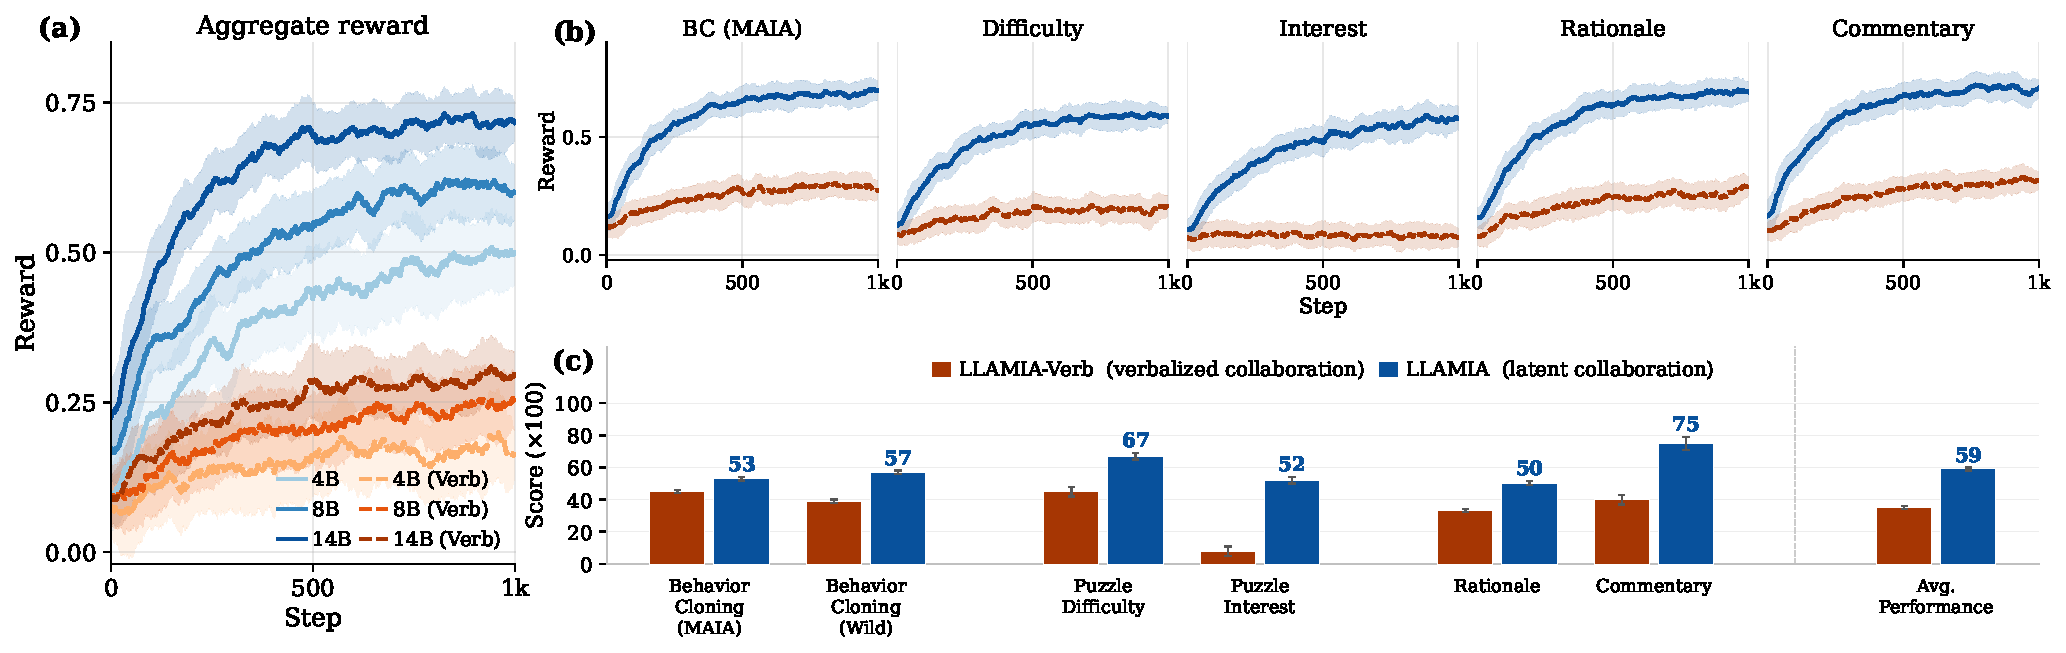
\includegraphics[width=\linewidth]{plots/combined_training_bench_verb_vs_llamia.pdf}
    \caption{%
    \textbf{DAPO training dynamics and LLAMIA-Bench evaluation.}
    \textbf{(a)}~Aggregate reward vs.\ training step at three backbone scales.
    Solid: LLAMIA (latent); dashed: LLAMIA-Verb (verbalized, identical recipe and backbone).
    The debt widens throughout and reaches $2$--$3\times$ by convergence; scaling the backbone does not close it for LLAMIA-Verb.
    \textbf{(b)}~Per-task reward curves at 14B.
    LLAMIA-Verb gains partial signal on behavior cloning and difficulty (tasks with verbalizable proxies) but stays near-flat on interest and commentary, where the reward requires non-verbalizable features or multi-step integration.
    \textbf{(c)}~LLAMIA-Bench scores ($0$--$100$).
    Puzzle Interest is diagnostic: every verbalized system scores ${\leq}12$ regardless of model scale or frontier capability, while LLAMIA-14B reaches $52$.
    Full per-task tables with confidence intervals in \cref{sec:app_results}.
    }
    \label{fig:combined}
\end{figure*}
LLAMIA-14B achieves the highest score on all six \textsc{LLAMIA-Bench} tasks (\cref{fig:combined}c), surpassing frontier verbalized systems an order of magnitude larger and remaining competitive with dedicated task-specific finetunes that are trained on substantially more in-domain data.
On behavior cloning, Maia and Allie are trained on tens of millions of chess-specific games, against LLAMIA's general-purpose backbone. LLAMIA-14B remains inside the expert band on the in-distribution Maia split and surpasses the strongest expert by a wide margin on the OOD Wild splits (GM-25, Low-Time, $\Delta$Elo), which probe regimes absent from the experts' blitz-only training mixture. Latent access to the engine's policy and value structure thus generalizes more reliably than direct supervision on a narrower distribution. Interest and commentary have no dedicated task-specific baseline at all, no published system predicts puzzle interestingness or generates grounded move commentary from engine state, which is itself evidence that these tasks require the joint reasoning LLAMIA provides rather than a narrower specialist.
The advantage over GPT-5\,+\,Lc0 does not require the 14B backbone: LLAMIA-8B already leads on all six tasks, and LLAMIA-4B on four of six (\cref{tab:full_bench}).
Per-task evaluations with additional metrics, baselines, and confidence intervals are in \cref{sec:app_results}.

\paragraph{Latent tokens enable new evaluation targets.}
Puzzle Interest requires ranking positions by community-derived interestingness, a signal that depends on the engine's policy distribution and value gradients across candidate moves.
No verbalized engine output carries these features.
Every verbalized system scores ${\leq}12$ on Interest regardless of model scale or frontier capability; LLAMIA-14B reaches $52$ (\cref{fig:combined}c).
Verbalization has zero useful signal for this task, while latent tokens give the LLM direct access to the distributional structure that defines interestingness.


% \begin{table}[t]
% \centering
% \caption{\textbf{LLAMIA-Bench summary and verbalization debt.}
% All scores normalized $0$--$100$; higher is better. LLAMIA and LLAMIA-Verb share the same 14B backbone, Lc0-BT4 subagent, and DAPO recipe; the only difference is the integration interface (latent tokens vs.\ verbalized text). The $\Delta$ row reports the \textbf{verbalization debt} per task. Task-specific expert is the strongest published baseline per task (Allie-Adaptive-Search for BC, SCC for Annotation); blanks indicate no dedicated baseline. Full per-scale factorial in \cref{tab:full_bench}.}
% \label{tab:main_bench}
% \begin{adjustbox}{max width=\columnwidth}
% \begin{tabular}{l|cc|cc|c|c}
% \toprule[1.2pt]
% \textbf{System} &
% \multicolumn{2}{c|}{\textbf{BC}} &
% \multicolumn{2}{c|}{\textbf{Puzzle}} &
% \textbf{Ann.} &
% \textbf{Comm.} \\
% & \textbf{MAIA} & \textbf{Wild} &
% \textbf{Diff.} & \textbf{Int.} & & \\
% \midrule
% Task-Spec. Expert  & \valbest{55} & 45 & -- & -- & 34.5 & -- \\
% GPT-5+Lc0         & 45 & 40 & 48 & 10 & 37.5 & 55 \\
% LLAMIA-Verb-14B   & 45 & 39 & 45 & 8 & 33.2 & 40 \\
% LLAMIA-14B        & 53 & \valbest{57} & \valbest{67} & \valbest{52} & \valbest{50.3} & \valbest{75} \\
% \midrule
% $\Delta$ (debt)   & $+8$ & $+18$ & $+22$ & $+44$ & $+17.1$ & $+35$ \\
% \bottomrule[1.2pt]
% \end{tabular}
% \end{adjustbox}
% \end{table}
% =========================================================================
\subsection{Verbalization Debt}
\label{sec:results_vd}
\somesh{Now that we have quantitatively differentiated LLAMIA on all tasks against Frontier + Task specific Finetunes we discuss the verbalization debt through key headings, first, define it. Summarize the results from table 1, then from figure Verbalization debt is consistent across scale, and throughout training, from training dynamics figure.}

LLAMIA and LLAMIA-Verb share the same 14B backbone, Lc0-BT4 subagent, and DAPO recipe; the only difference is whether the subagent's state reaches the LLM as latent tokens or as verbalized text. We define the resulting performance gap as the \textbf{verbalization debt}.

\paragraph{Verbalization debt is significant across all tasks}
Figure \ref{fig:combined} shows that the verbalization debt is consistent across all six tasks. The gap is largest on Interest and Commentary, where the target signal lives in the engine's full policy distribution or value landscape and has no faithful text equivalent, and smallest on in-distribution behavior cloning, where the engine's top-$k$ moves already approximate the answer and the verbal summary loses little.

\paragraph{The debt persists across backbone scale.}
Increasing the LLM from 4B to 14B improves both systems, but the debt persists at every scale (\cref{tab:full_bench}). On Interest, LLAMIA-Verb-14B scores $8$ while LLAMIA-4B already reaches $38$.

\paragraph{The debt widens throughout training.}
The debt grows throughout DAPO, reaching $2$--$3\times$ by the end of training (\cref{fig:combined}a). Per-task reward curves (\cref{fig:combined}b) reveal where the verbal channel saturates: LLAMIA-Verb gains partial signal on behavior cloning and difficulty, where the verbalized output carries a useful proxy (top-$k$ moves, solution length), but stays near-flat on interest and commentary, where no such proxy exists.

\subsection{Ablations}
\label{sec:results_ablations}
To further understand the verbalization debt and isolate the contribution of internalization and reinforcement learning we conduct the following ablations and compare in \cref{tab:ablation_main}. \textbf{LLM-Only} trains with RL but no engine, so any gain has to come from the weights. \textbf{LLM-ChessCLIP} trains with RL and the same $32$ latent slots as LLAMIA, but filled by a raw board encoder (ChessCLIP, a PaLM-E-style injection) rather than Lc0's state, so any gain has to come from capacity rather than content. \textbf{Qwen3+Lc0 (untr.)} is untrained tool use. \textbf{LLAMIA-Verb} is RL on top of verbalized text. \textbf{LLAMIA-SFT (latent)} removes RL, the reasoning trace, and the invocation policy, leaving only the latent channel. \textbf{LLAMIA} is the full system. Extended controls, latent-only, shuffled tokens, per-task probes, and templates, are in \cref{sec:abl_interface,sec:app_baselines_probe}.

\begin{table}[t]
\centering
\caption{\textbf{Interface controls} (14B). BC in \% move-match; Difficulty and Interest in Spearman $\rho$; Rationale in BLEU-2; Commentary in G-eval. All trained systems share backbone, data, and recipe; only the interface differs.}
\label{tab:ablation_main}
\begin{adjustbox}{max width=\columnwidth}
\renewcommand{\arraystretch}{1.15}
\small
\begin{tabular}{lcccccc}
\toprule[1.2pt]
\textbf{System} & \textbf{BC-M} & \textbf{BC-W} & \textbf{Diff.} & \textbf{Int.} & \textbf{Rat.} & \textbf{Comm.} \\
\midrule
LLM-Only (RL, no engine)          & $34$ & $19$ & $0.22$ & $0.07$ & $16.1$ & $0.13$ \\
LLM-ChessCLIP (RL, raw encoder)   & $39$ & $28$ & $0.24$ & $0.08$ & $23.1$ & $0.29$ \\
Qwen3\,+\,Lc0 (untr.\ tool use)   & $39$ & $33$ & $0.28$ & $0.05$ & $18.8$ & $0.15$ \\
LLAMIA-Verb (RL, text only)       & $45$ & $39$ & $0.45$ & $0.08$ & $33.2$ & $0.40$ \\
LLAMIA-SFT (latent, no RL)        & $51$ & $46$ & $0.66$ & $0.48$ & $38.5$ & $0.58$ \\
LLAMIA (latent, RL)               & \valbest{$53$} & \valbest{$49$} & \valbest{$0.71$} & \valbest{$0.52$} & \valbest{$45.8$} & \valbest{$0.75$} \\
\bottomrule[1.2pt]
\end{tabular}
\end{adjustbox}
\vspace{-3mm}
\end{table}

\paragraph{The gain comes from Lc0's latent state, not from weights or capacity.}
LLM-Only and LLM-ChessCLIP get the same RL recipe as LLAMIA and still land near or below untrained tool use, so DAPO cannot manufacture the missing expertise on its own, whether it is asked to bake it into the weights or to make sense of $32$ slots filled with the wrong content. Shuffling LLAMIA's own latent tokens produces the same collapse toward LLAMIA-Verb even though the token count never changes (\cref{sec:abl_interface}). The pattern only breaks when those slots carry Lc0's own policy and value representations. Further, LLAMIA-SFT, with no RL recovers most of the verbalization debt. However, it compounds the effect of internalization by bringing the improvements in multi step strategies, where the model has to plan across latent states i.e. Game Commentary and Rationale generation. We further show this through the emergent latent collaboration strategies in \cref{sec:results_agency}.

\subsection{Collaboration Strategies}
\label{sec:results_agency}
\somesh{The signposting or motivation of why we are discussing Collaboration strategies is missing. `apart from quantitative comparison in agent performance we now analyze the learnt collaboration strategies through internalization and RL over multi-step planning. We qualitatively analyze and identify the following dominant patterns of subagent invokation and actions as shown in figure 2. We describe these patterns and their definitions in appendix ... Then key headlines, training for strategic collaboration with non language agent collapses with verbalization, whereas with internalization LLAMIA exhibits better agency with task specific strategies learnt during training. Defer to dynamics from figure only.}
Does the integration interface determine how the model learns to use the subagent, or only how well it performs? We classify subagent invocations during evaluation into five recurring strategies and trace their evolution during DAPO training (\cref{fig:agency_task_specificity}; strategy definitions and per-task heatmaps in \cref{fig:agency_heatmaps}).

\begin{figure}[t]
    \centering
    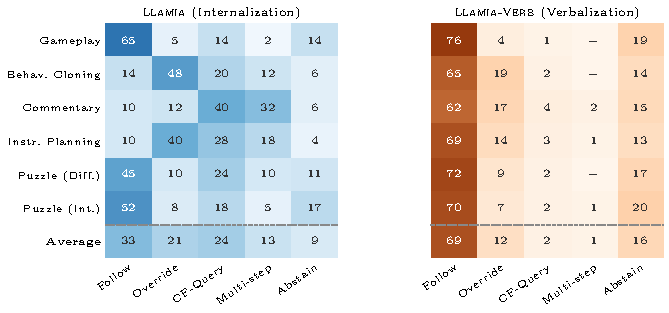
\includegraphics[width=\linewidth]{pages/figures/agency_strategy_heatmaps.pdf}
    \caption{\textbf{Collaboration strategy distribution (\%) per task at convergence.}
  Fraction of 500 episodes assigned to each strategy by a GPT-4o judge
  ($\kappa{=}0.78$). \emph{Left:} LLAMIA (latent). \emph{Right:} LLAMIA-Verb
  (verbalized). LLAMIA's dominant strategy shifts with the task
  (engine-follow for gameplay, consult-then-override for BC, counterfactual
  query for commentary); LLAMIA-Verb collapses to engine-follow on every
  row (62--76\%). Detailed discussion can be found in \cref{sec:abl_agency_strategies}}
    \label{fig:agency_heatmaps}

    \vspace{-2mm}
\end{figure}


The five strategies are \emph{engine-follow} (adopt the top recommendation), \emph{consult-then-override} (query then diverge), \emph{counterfactual query} (play a hypothetical move, re-invoke, compare states), \emph{multi-step lookahead} (chain two or three counterfactual sequences), and \emph{abstention} (act from language knowledge alone). A GPT-4o judge classifies 500 episodes per task per system ($\kappa{=}0.78$ vs.\ human raters).

\paragraph{Internalization produces task-specific collaboration; verbalization collapses it.}
LLAMIA adapts its strategy to the task: engine-follow dominates gameplay (65\%), consult-then-override dominates behavior cloning (48\%), and counterfactual query dominates commentary (40\%). LLAMIA-Verb collapses to engine-follow on every task (62--76\%), regardless of what the task requires (\cref{fig:agency_heatmaps}). The verbalized channel returns the same compressed summary no matter how the model queries it, so RL converges on a single use pattern.

\paragraph{The learned strategy makes internalization inference-cost neutral.}
Because it reasons over the full latent state, LLAMIA learns to invoke the subagent less often than LLAMIA-Verb ($1.9$ vs.\ $2.9$ calls per query at 14B). Each latent invocation adds a fixed $32$ tokens ($182$ vs.\ $150$), but the lower call count offsets this, so average tokens-per-query and wall-clock latency are comparable or lower than the verbalized interface; training cost stays within ${\sim}6\%$ of the verbalized pipeline at every scale (\cref{sec:app_cost}). Latent internalization therefore does not trade accuracy for inference cost.

\subsection{Human Evaluation}
\label{sec:results_human}

\begin{figure*}[t]
    \centering
    \begin{subfigure}[t]{0.235\linewidth}
        \centering
        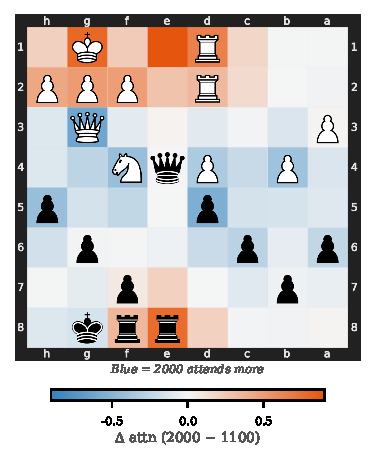
\includegraphics[width=\linewidth]{pages/figures/board_heatmap_c4_diff.pdf}
        \label{fig:human_heatmap}
    \end{subfigure}\hfill
    \begin{subfigure}[t]{0.245\linewidth}
        \centering
        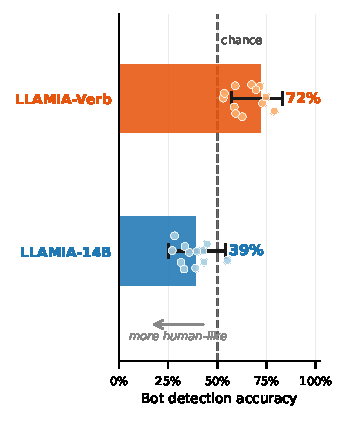
\includegraphics[width=\linewidth]{pages/figures/llamia_human_gameplay_compact.pdf}
        \label{fig:human_gameplay_main}
    \end{subfigure}\hfill
    \begin{subfigure}[t]{0.245\linewidth}
        \centering
        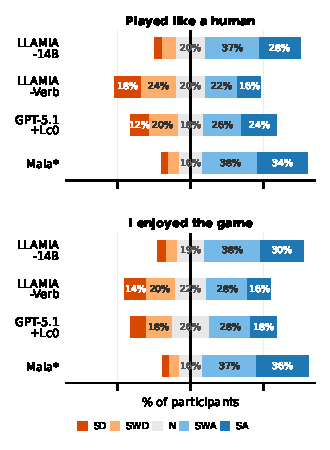
\includegraphics[width=\linewidth]{pages/figures/llamia_survey_vert.pdf}
        \label{fig:human_survey_main}
    \end{subfigure}\hfill
    \begin{subfigure}[t]{0.245\linewidth}
        \centering
        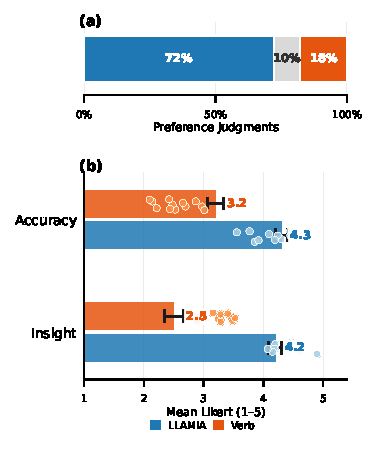
\includegraphics[width=\linewidth]{pages/figures/llamia_human_commentary_compact.pdf}
        \label{fig:human_commentary_main}
    \end{subfigure}
    \vspace{-4mm}
    \caption{%
    \textbf{Human evaluation ($n{=}12$ skilled players, all rated ${\geq}1700$).}
    \textbf{(a)}~Attention difference over latent tokens on a back-rank mate position: conditioning on 2000~Elo concentrates attention on mating geometry (red); 1100~Elo disperses to material (blue). The same latent state is read differently depending on the language instruction.
    \textbf{(b)}~Bot-detection rate (Study~1): LLAMIA-14B passes as human in 61\% of trials (detection 39\%, below chance); LLAMIA-Verb detected in 72\%.
    \textbf{(c)}~Post-game Likert (Strongly Disagree $\rightarrow$ Strongly Agree): LLAMIA matches Maia* (best Maia variant per Elo bucket) on human-likeness without training on human-move distributions.
    \textbf{(d)}~Commentary preference (Study~2): 72.2\% of 180 judgments favour LLAMIA; Insight gap (1.7\,pts) exceeds Accuracy gap (1.1\,pts).
    Study design and qualitative results in \cref{sec:app_human}.
    }
    \vspace{-3mm}
    \label{fig:human_eval}
\end{figure*}

\paragraph{Gameplay.}
Skilled players ($n{=}12$, all ${\geq}1700$ Elo) cannot reliably distinguish LLAMIA from a human opponent: detection falls below chance (\cref{fig:human_gameplay_main}), and post-game ratings place LLAMIA alongside Maia* on perceived human-likeness (\cref{fig:human_survey_main}). Maia is trained directly on millions of move distributions; LLAMIA receives no human-move supervision. Instead, behavioral signatures such as time-pressure blunders and skill-appropriate piece saliency emerge from latent-state conditioning alone. LLAMIA-Verb, trained with the same backbone and DAPO budget, is detected at rates well above chance, consistent with the stylistic regularities that verbal summaries impose on move selection.

\paragraph{Commentary.}
Both systems achieve comparable factual accuracy: material balance, initiative assessment, and basic evaluations survive verbalization reasonably well. The gap concentrates on strategic insight (\cref{fig:human_commentary_main}), where participants rate LLAMIA higher by a wider margin on the Insight dimension than on Accuracy. Text preserves \emph{what} is happening on the board, but explaining \emph{why} a move is strong requires representational features (policy gradients, value topology, look-ahead depth) that do not survive verbal compression.

\paragraph{Latent tokens are instruction-modulated.}
On a fixed back-rank mate position (\cref{fig:human_heatmap}), LLAMIA's attention over the latent tokens shifts with the target Elo: at 2000 it concentrates on the mating geometry, at 1100 it disperses to material. The latent representation is identical in both cases; what changes is the LLM's reading, conditioned on the natural-language Elo instruction. The projected state functions as a perceptual input shaped by task context, not a static feature vector.

\subsection{Generalization Beyond Chess}
\label{sec:results_go}

To provide initial evidence that LLAMIA can transfer beyond chess, we instantiate it on Go. We use KataGo-b18~\cite{wu2019katago}, a state-of-the-art Go neural engine, as the non-language subagent. We train a three-layer LatentBridge, with the first-layer width matched to KataGo's $384$ trunk channels and the $361$ board intersections represented as spatial tokens, using the same two-stage DAPO procedure on rank-conditioned behavior cloning. LLAMIA-Go-$14$B achieves $48$/$50$ top-1 human move-match at ranks 5k/5d using only $8$k positions, matching the rank-calibrated KataGo-HumanSL expert~\cite{wu2024katagohuman} and outperforming the verbalized control by ${\sim}10$ points. The latent-over-verbal gap remains consistent across the 4B, 8B, and 14B model scales (\cref{sec:app_go}). These results provide strong evidence that latent collaboration is not specific to chess. Establishing broader generality across environments and task families remains an important direction for future work.